
\chapter*{Questão 3}

\section*{Enunciado}
\noindent
3. Considere agora o caso do andarilho bidimensional não enviesado, i.e., com iguais chances $\left(\frac{1}{4}\right)$ ele dá um passo em qualquer direção dos pontos cardeais: norte, sul, leste e oeste. Calcule $\langle \vec{r} \rangle$ e 
$\Delta^2 = \langle \vec{r} \cdot \vec{r} \rangle - \langle \vec{r} \rangle \cdot \langle \vec{r} \rangle$.
Repare que estes andarilhos perfazem o mesmo tipo de movimento que moléculas no processo de difusão, como por exemplo a difusão de um pingo de leite numa xícara de café. Faça um diagrama das posições das moléculas após um número $N$ de passos 
$(N = 10, 10^2, 10^3, 10^4, 10^5, 10^6)$.

\section*{Metodologia}
Nesse problema, é pedido para generalizar o caso do andarilho aleatório das simulações \textbf{2A} e \textbf{2B} para o plano 2D, portanto, o código criado é similar ao da questão \textbf{2}. Vale notar que, ao contrário do problema anterior, nesse problema, o andarilho tem igual chance de caminhar na direção norte, sul, leste e oeste, ou seja, a probabilidade dele dar um passo em cada uma dessas direções é 1/4.

\section*{Código}
O programa \texttt{main} é responsável por chamar a função \texttt{calc(m,n)} com 
os parâmetros $m=10^2$ (número de caminhantes) e $n=10^3$ (número de passos de cada caminhante). 
A função \texttt{calc} implementa o movimento de andarilhos bidimensionais (caminhantes aleatórios), 
que dão passos em direções norte, sul, leste ou oeste com probabilidades iguais 
($\tfrac{1}{4}$ cada). O objetivo é calcular as quantidades 
$\langle \vec{r} \rangle$, $\langle \vec{r}\cdot \vec{r} \rangle$ e 
$\langle (\Delta r)^2 \rangle = \langle \vec{r}\cdot \vec{r} \rangle - \langle \vec{r}\rangle \cdot \langle \vec{r}\rangle$, 
bem como salvar a distribuição final das posições em um arquivo externo.  

Logo no início da função, define-se \texttt{iseed=12}, a semente do gerador pseudo-aleatório. 
A chamada \texttt{rr = rand(iseed)} inicializa a sequência de números aleatórios.  
Em seguida, é criado o vetor \texttt{istep(1:2)} com os possíveis incrementos de posição: 
$+1$ e $-1$. O array bidimensional \texttt{ipos(-n:n,-n:n)} é inicializado com zeros, 
sendo ele responsável por registrar a frequência de caminhantes que terminaram em cada posição $(i,j)$ 
do reticulado bidimensional.  

A etapa principal do cálculo ocorre em dois laços aninhados:  
(i) para cada um dos $m$ caminhantes, inicializa-se a posição em $(0,0)$;  
(ii) em cada um dos $n$ passos, sorteia-se uma direção usando o par de variáveis 
\texttt{idir} e \texttt{irand}.  
O valor \texttt{idir = 2e0*rand()} (truncado para 0 ou 1) decide se o passo ocorrerá 
no eixo $x$ ou no eixo $y$, enquanto \texttt{irand = 2e0*rand() + 1} escolhe o sentido 
(índice para \texttt{istep}), resultando em $+1$ ou $-1$.  
Ao final dos $n$ passos, o contador \texttt{ipos(ix,iy)} é incrementado, armazenando 
quantos caminhantes terminaram na posição $(ix,iy)$.  

Com a distribuição final das posições construída, o código calcula primeiro o vetor médio 
$\langle \vec{r} \rangle$. Isso é feito somando-se todas as posições finais $(i,j)$ ocupadas 
(pesadas pela frequência em \texttt{ipos}) e dividindo pelo número de caminhantes $m$. 
Em seguida, calcula-se $\langle \vec{r}\rangle \cdot \langle \vec{r}\rangle = r_1$.  

Depois, a função calcula $\langle \vec{r}\cdot \vec{r}\rangle = r_2$, obtido pela soma dos 
quadrados das coordenadas $(i^2+j^2)$ de todas as posições finais ocupadas, também dividido por $m$.  
A diferença entre $r_2$ e $r_1$ fornece o desvio quadrático médio:  
\[
\langle (\Delta r)^2 \rangle = \langle \vec{r}\cdot \vec{r} \rangle - \langle \vec{r}\rangle \cdot \langle \vec{r}\rangle.
\]  

Por fim, os resultados são gravados em um arquivo \texttt{saida-1-12694394.txt}, 
onde cada linha contém as coordenadas finais $(i,j)$ e a frequência \texttt{ipos(i,j)} 
de caminhantes que terminaram naquela posição. O formato usado é \texttt{I4,',',I4,',',I4}, 
permitindo futura análise gráfica ou estatística da distribuição espacial.  

Em resumo, esse programa realiza a simulação de um conjunto de caminhantes aleatórios 
em duas dimensões, calcula grandezas médias associadas ao processo de difusão 
($\langle \vec{r} \rangle$, $\langle r^2 \rangle$, $\langle (\Delta r)^2 \rangle$) 
e armazena a distribuição final das posições em arquivo para inspeção posterior.  

\vspace*{1\baselineskip}

\begin{figure}[h!]
\centering
\caption{Função principal do código.}
\centering
\begin{lstlisting}
program main
    n = 3000
    m = 1000
    x = calc(m,n)
end program main
\end{lstlisting}
\caption*{Fonte: Compilado pelo Autor.}
\label{fig:tarefa 3 - função principal do código}
\end{figure}

\newpage

\begin{figure}[h!]
\centering
\caption{Função que realiza os cálculos.}
\centering
\begin{lstlisting}

function calc(m,n)
parameter(iseed=12)
dimension istep(1:2), ipos(-n:n,-n:n)

! Da o seed para o rand()
rr = rand(iseed)

! Inicia o vetor istep
istep(1) = 1
istep(2) = -1

! Inicia o vetor posição
do i =-n,n
    do j = -n,n
        ipos(i,j) = 0
    end do
end do

! Cálculos
ixm = 0
iym = 0
do i =1,m
    ix = 0
    iy = 0
    do j = 1,n
        ! Escolho se vou na direção x ou y
        idir = 2e0*rand()
        irand = 2e0*rand() + 1
        if (idir .EQ. 0) then
            ix = ix + istep(irand)
        else
            iy = iy + istep(irand)
        end if
    end do
    ipos(ix,iy) = ipos(ix,iy) + 1
end do

\end{lstlisting}
\caption*{Fonte: Compilado pelo Autor.}
\label{fig:tarefa 3 - função principal do código}
\end{figure}

\newpage

\begin{figure}[H]
\centering
\caption{continuação da função que realiza os cálculos.}
\centering
\begin{lstlisting}

        ! Cálcula o valor médio da posição <r>
        r1x = 0
        r1y = 0
        do i =-n,n
            do j =-n,n
                if (ipos(i,j) .NE. 0) then
                    r1x = r1x + i
                    r1y = r1y + j
                end if
            end do
        end do
        r1x = r1x/m
        r1y = r1y/m
        rr1 = r1x + r1y
        r1 = (r1x*r1x) + (r1y*r1y)

        ! Cálcula o valor médio de <r.r>
        r2=0
        do i =-n,n
            do j =-n,n
                if (ipos(i,j) .NE. 0) then
                    r2 = r2 + (i*i) + (j*j)
                end if
            end do
        end do
        r2 = r2/m

        ! Calcula o valor de <(delta_r)^2> = <r.r> - <r>.<r>
        dr2 = r2 - r1

        ! Escreve na tela <(delta_r)^2> e <r>
        write(*,*)" <r>, <(delta_r)^2>"
        write(*,11) rr1,dr2
        ! Salva os resultados
        open(unit=1,file='saida-1-12694394.txt')
        do i =-n,n
            do j = -n,n
            if (ipos(i,j) .GT. 0) then
                write(1,7) i,j,ipos(i,j)
            end if
            end do
        end do
7       format(I4,',',I4,',',I4)
11      format(F12.4, F12.4)
        close(1)
        end function calc
\end{lstlisting}
\caption*{Fonte: Compilado pelo Autor.}
\label{fig:tarefa 3 - função principal do código}
\end{figure}


\newpage
\section*{Resultados e Discussão}

Nesta seção, serão exibidos os dados resultados obtidos através da simulação da tarefa 3,
nas Figuras - \ref{fig:tarefa 3 - Primeiro histograma} e \ref{fig:tarefa 3 - Segundo histograma}
são contemplados as posições de 1000 caminhantes aleatórios dando 3000 passos. Desses gráficos,
fica evidente que a tendencia é que após 3000 passos que podem ser para qualquer direção do eixo cardial,
e sem preferencia para uma direção, o andarilho tende a ficar na sua posição inicial, no nosso caso (0,0).
Ademais, na Tabela - \ref{table:tabela_2} são apresentados os valores da média $\langle r \rangle$ e $ \Delta^2 $
para diferentes números de passos, \textit{n}, nela é visível que quanto maior o número de passos, maior é o valor do desvio padrão e 
o valor de $\langle r \rangle$ tende a 0. 

\vspace*{1\baselineskip}

\begin{table}[h!]
\centering
\caption{Valores da média $\langle r \rangle$ e $ \Delta^2 $ para diferentes números de passos, \textit{n}, com o número de andarilhos fixo igual a $m = 1000$}
\begin{NiceTabular}
   [
     columns-width=3cm,
     hvlines-except-borders,
     rules={color=white,width=1pt}
   ]
   {ccc}
\CodeBefore
  \rowcolor{cyan}{1}
  \rowcolors{2}{cyan!25}{cyan!15}
\Body
  \RowStyle[color=white]{}
  \textit{n} & $\langle r \rangle$ & $ \Delta^2$ \\
  1000 & -1.5580 & 930.8069   \\
  2000 & -2.6220 & 1931.1337 \\
  3000 & -1.5500 & 2891.0312 \\
  4000 & -0.3080 & 3876.8213 \\
  5000 & -0.0760 & 4862.9712 \\
\end{NiceTabular}
\caption*{Fonte: Compilado pelo Autor}
\label{table:tabela_2}
\end{table}

\begin{figure}[h!]
\centering
  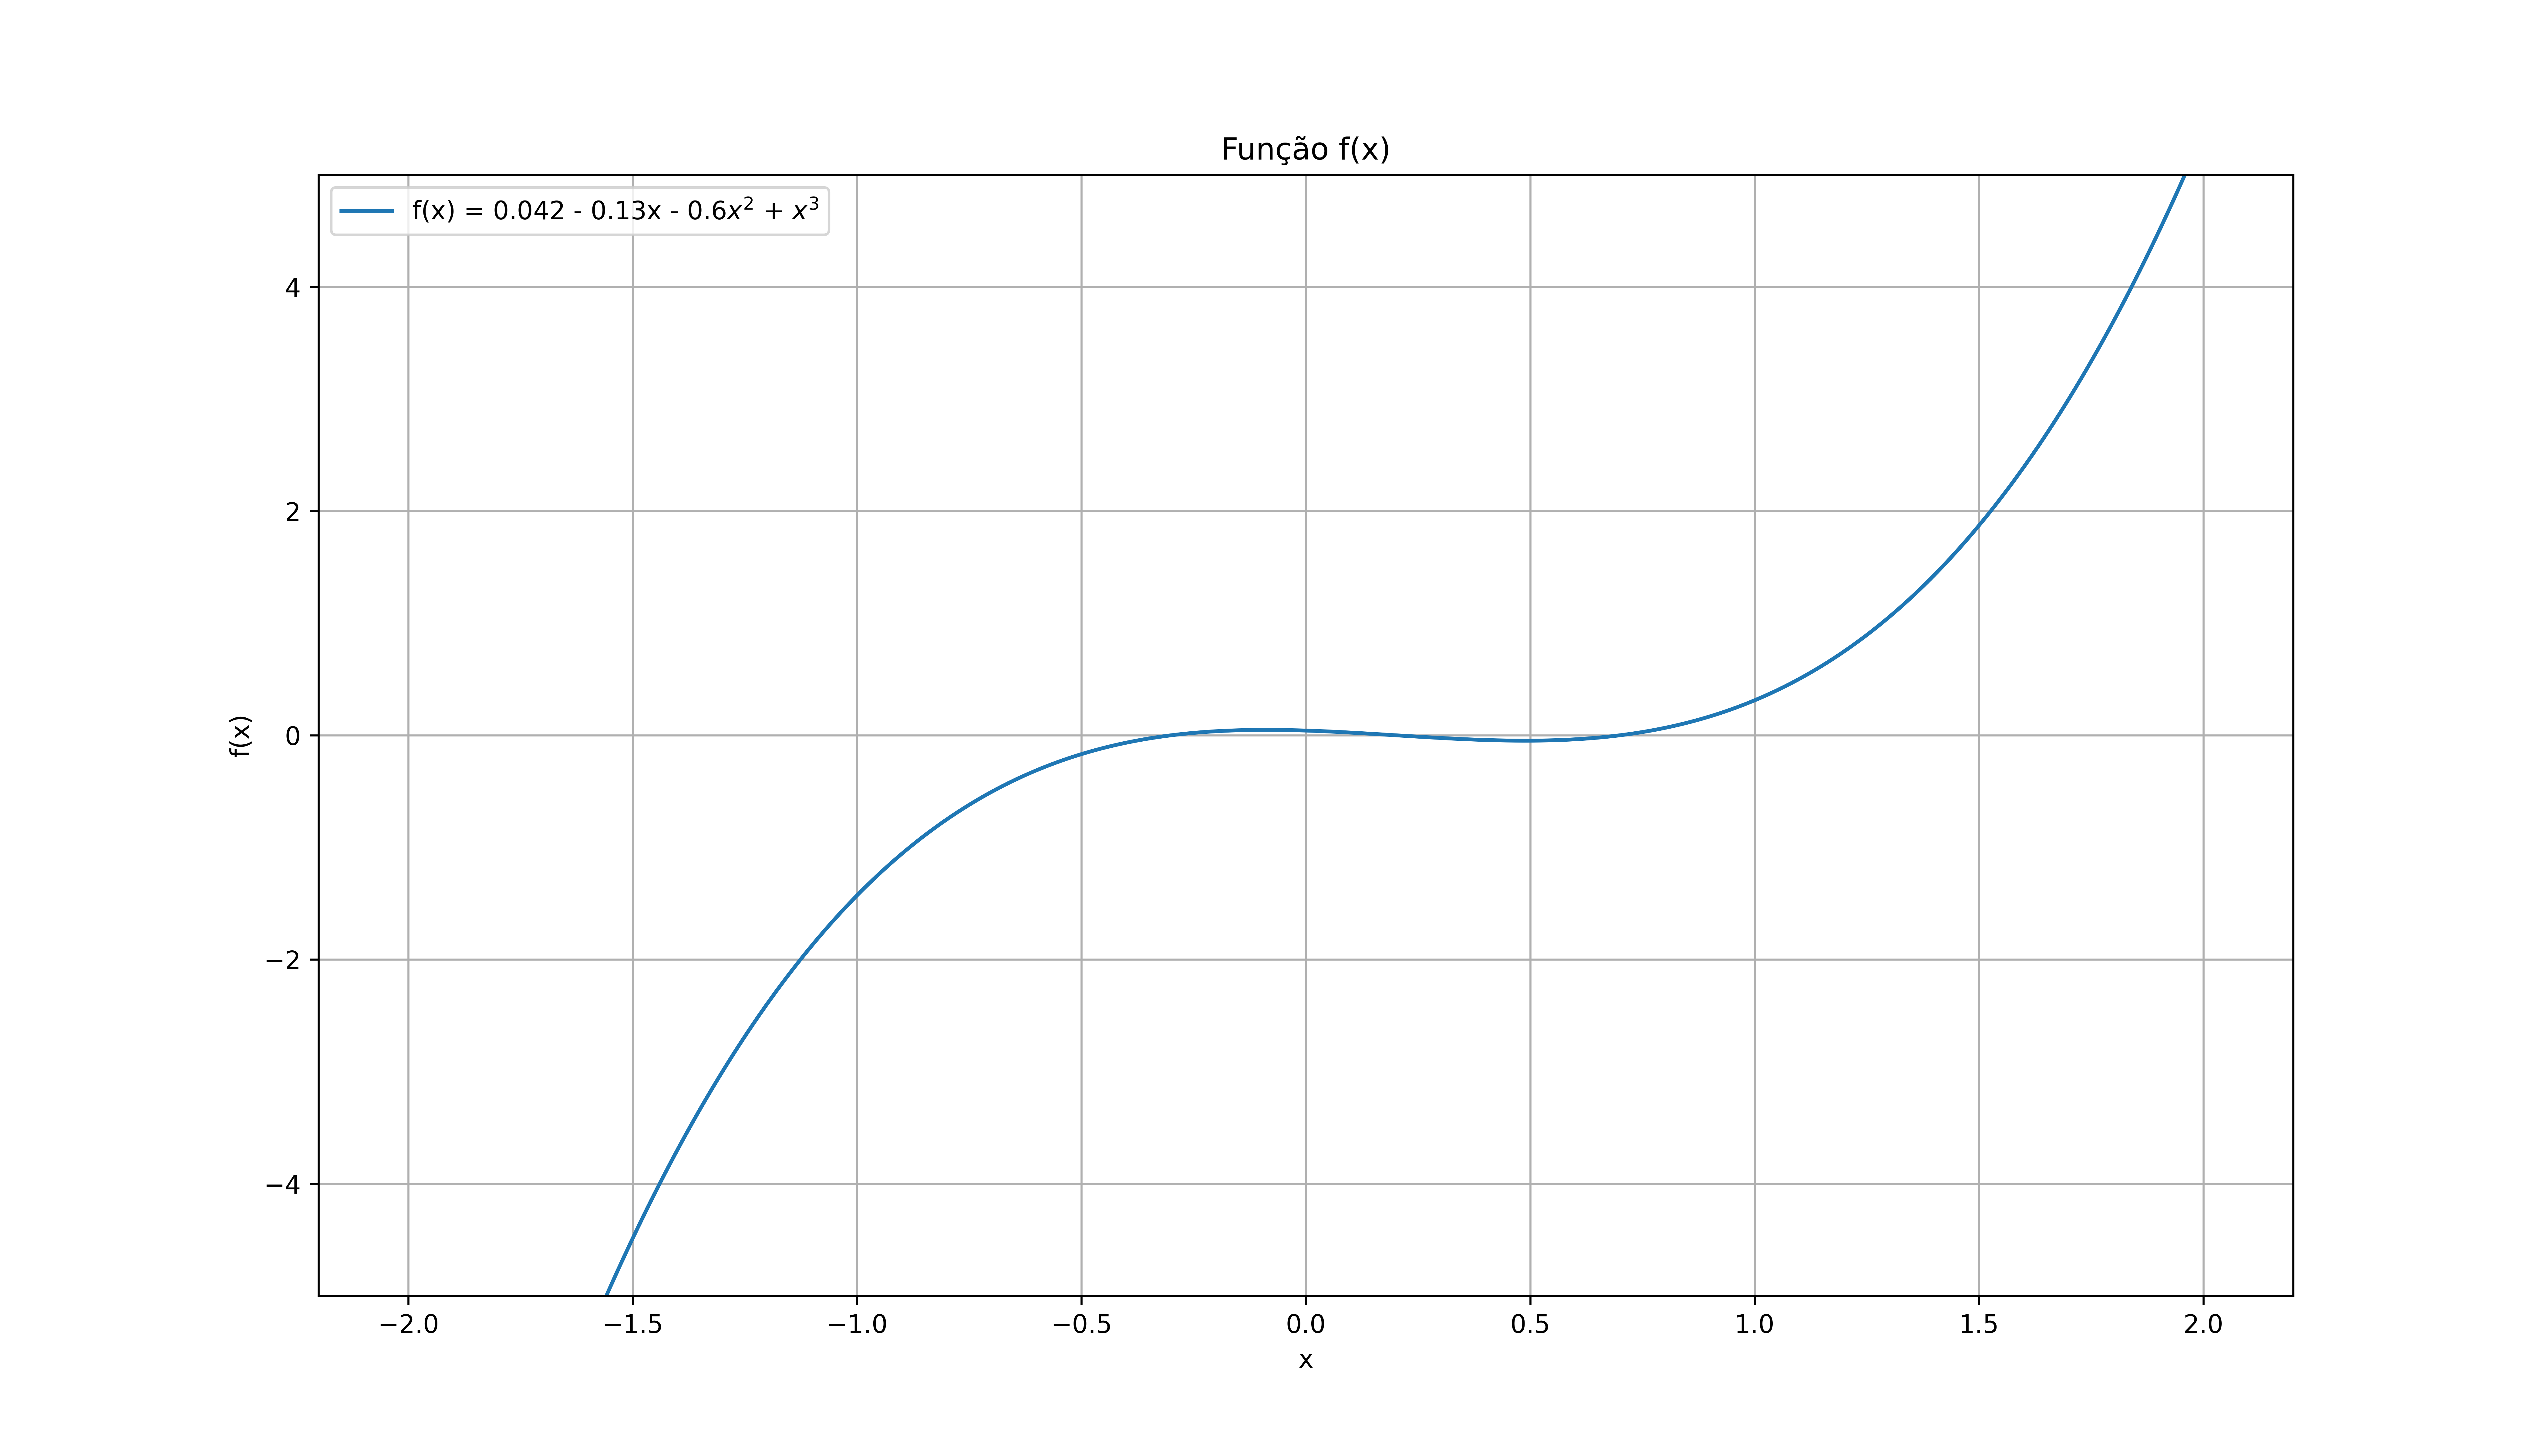
\includegraphics[width=16cm]{images/tarefa-3/tarefa-3-graf-1.png}
  \caption{Histograma 2D da posição dos caminhantes aleatórios no eixo xy.}
\caption*{Fonte: Compilado pelo Autor.}
\label{fig:tarefa 3 - Primeiro histograma}
\end{figure}

\begin{figure}[h!]
\centering
  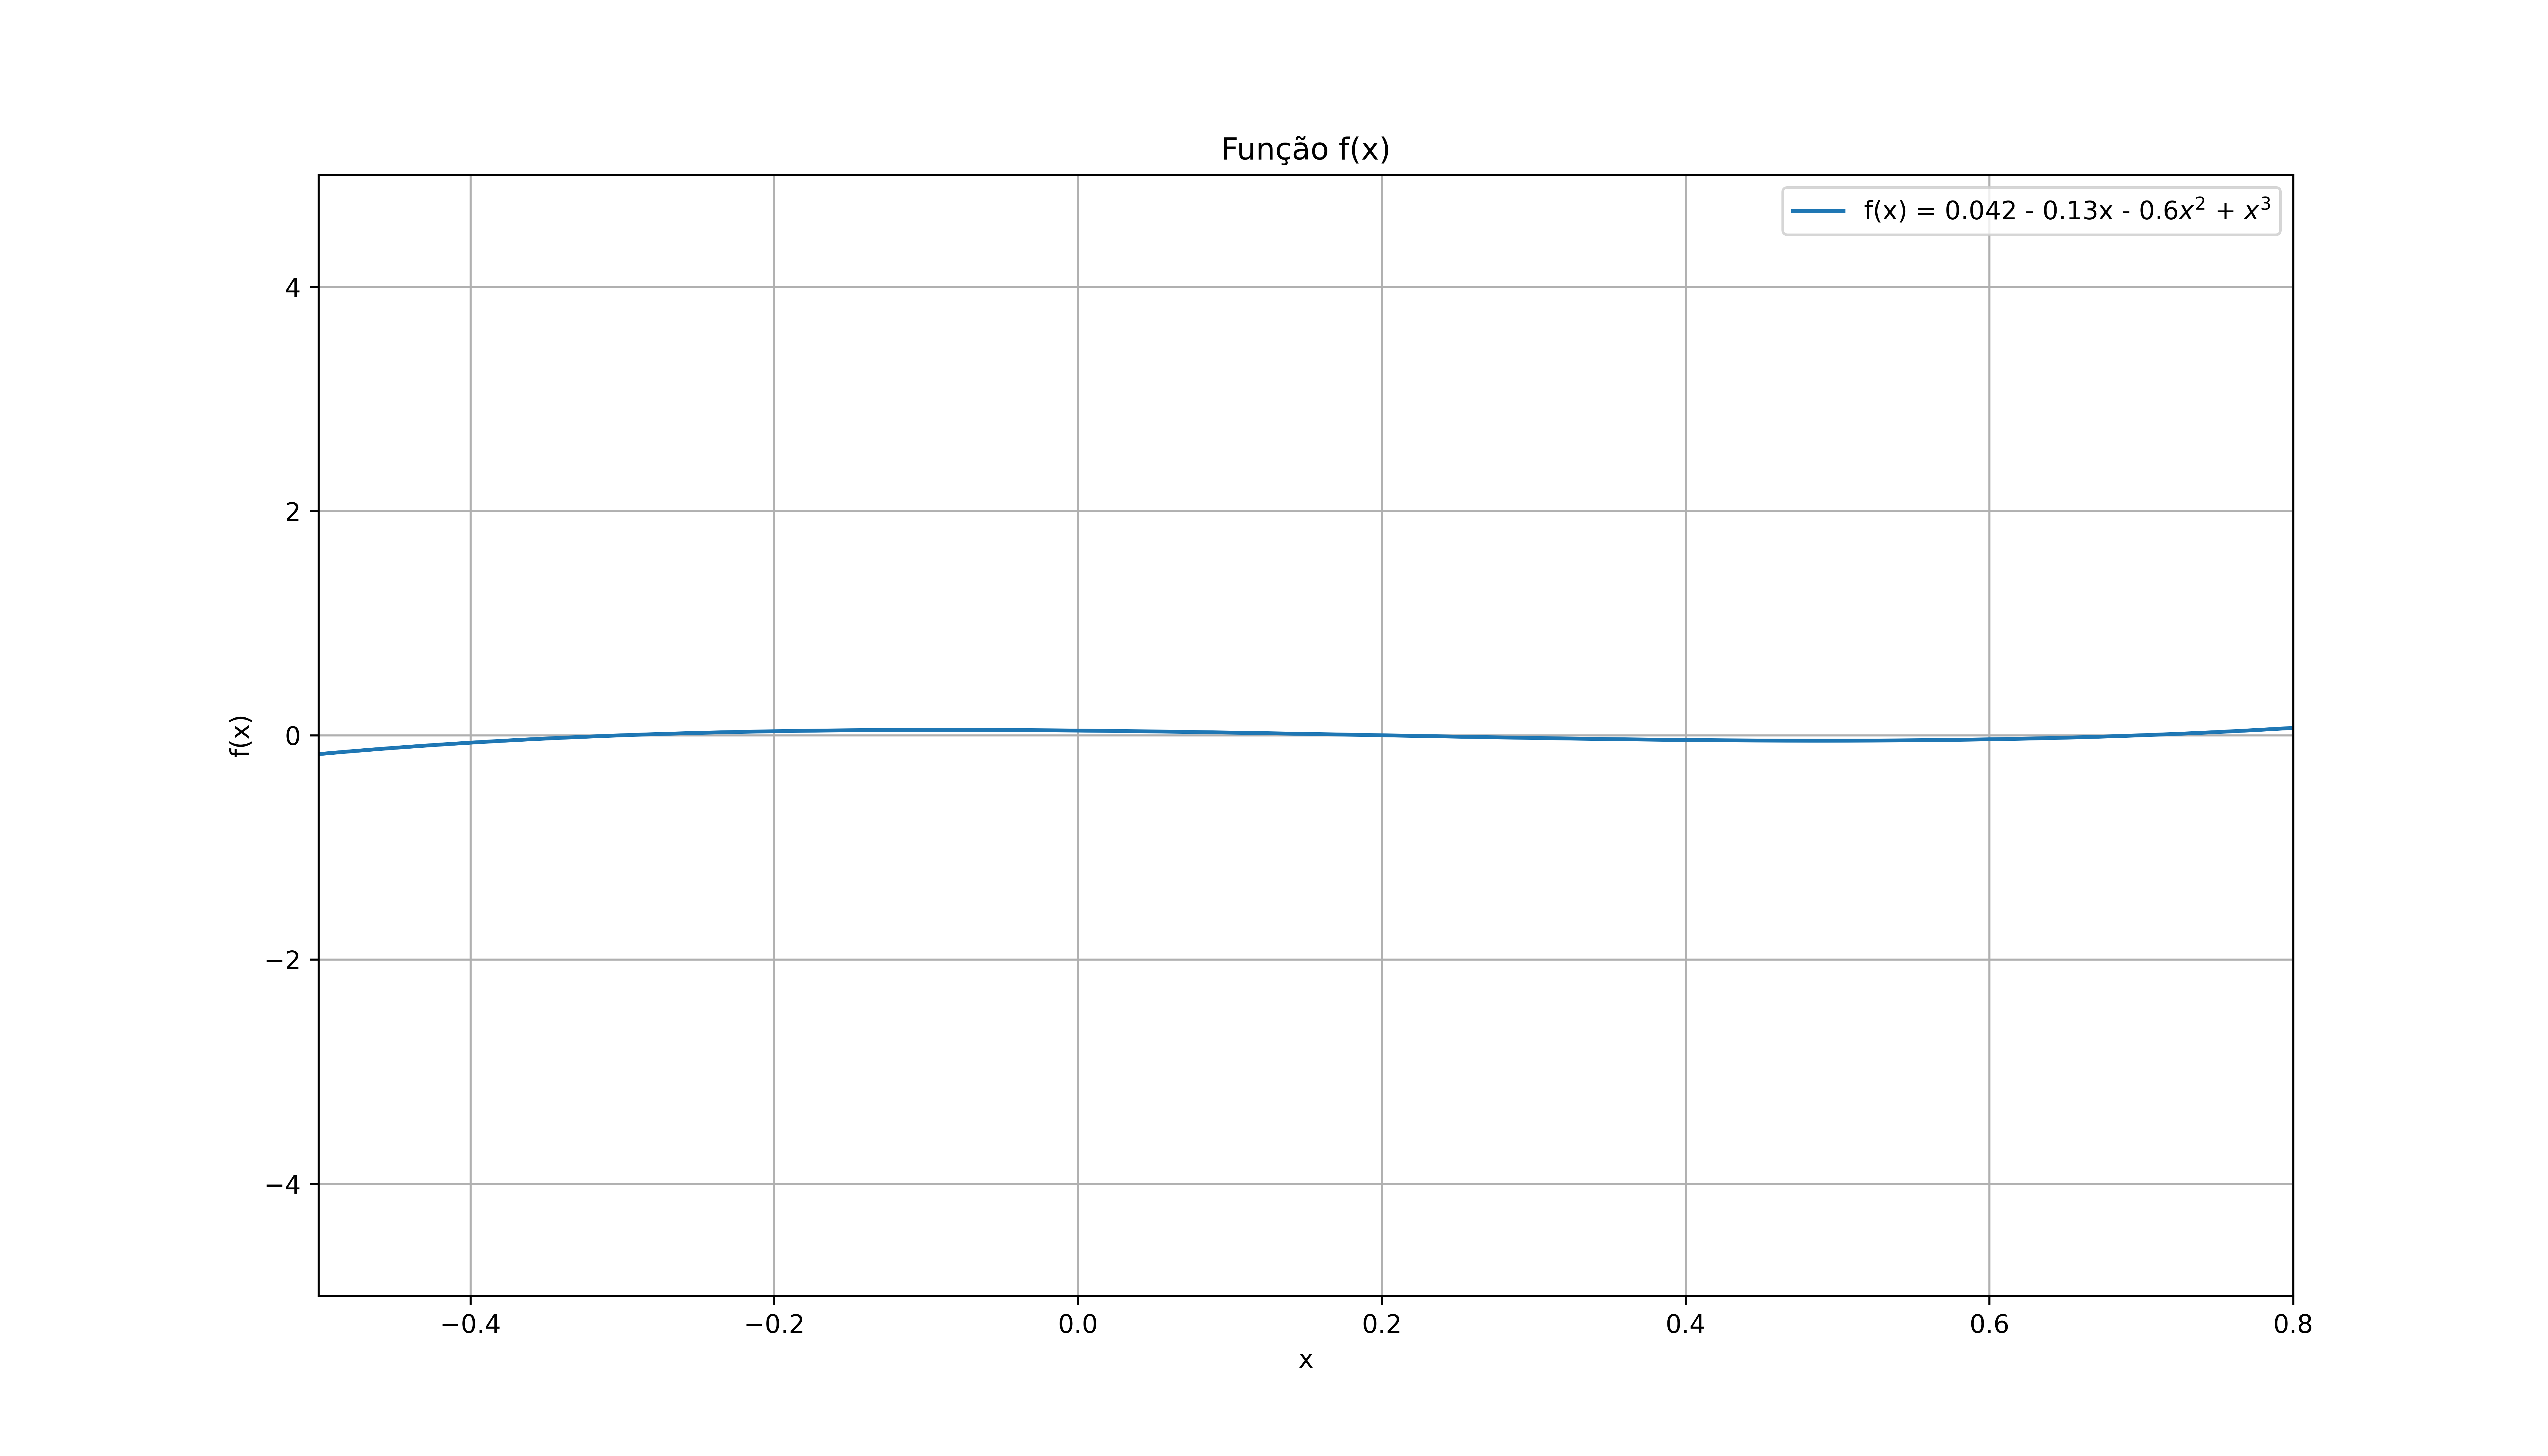
\includegraphics[width=16cm]{images/tarefa-3/tarefa-3-graf-2.png}
  \caption{Histograma 2D da posição dos caminhantes aleatórios no eixo xy, nas margens são histogramas
  da distribuição de caminhates aleatórios em cada eixo.}
\caption*{Fonte: Compilado pelo Autor.}
\label{fig:tarefa 3 - Segundo histograma}
\end{figure}


\begin{figure}[h!]
\centering
\caption{Resultado exibido pela simulação no terminal, onde os valores forem de $m=1000$ e $n=5000$.}
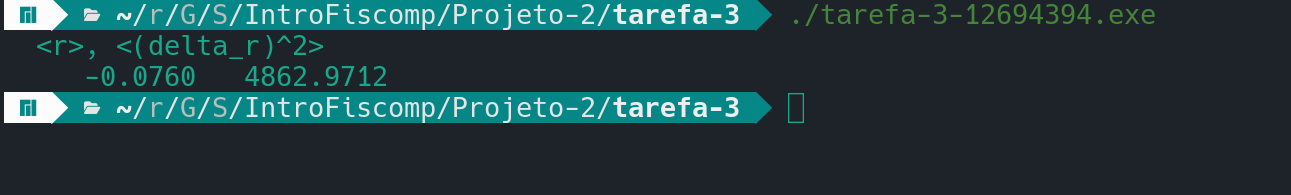
\includegraphics[width=16cm]{images/tarefa-3/terminal.png}
\caption*{Fonte: Compilado pelo Autor.}
\label{fig:tarefa 3 - terminal}
\end{figure}
